\documentclass[12pt]{article}

\usepackage[T1]{fontenc}
\usepackage{textcomp}

\usepackage[english]{babel}
\usepackage[utf8]{inputenc}

\usepackage{lmodern}

\usepackage{hyperref}
\hypersetup{breaklinks}
\hypersetup{pdfborder=0 0 0}

\usepackage[babel=true]{microtype}


\usepackage{amsmath}
\renewcommand{\vec}[1]{\mathbf{#1}}
\newcommand{\mat}[1]{\mathbf{#1}}
\DeclareMathOperator{\Prob}{Prob}
\DeclareMathOperator{\diag}{diag}
\newcommand{\md}{\mathrm{d}}
\newcommand{\me}{\mathrm{e}}
\newcommand{\mT}{\mathrm{T}}

\usepackage{units}
\usepackage{tikz}
\usepackage{natbib}
\usepackage{hypernat}

\allowdisplaybreaks[1]

\title{Supplementary Material for\\
  \emph{Interactions between chronic diseases: asymmetric outcomes of
    co-infection at individual and population scales} \\
  Appendix 3: Model development and analysis}

\author{Anna Jolles \and Erin Gorsich \and Simon Gubbins
  \and Brianna Beechler \and Peter Buss \and Bryan Charleston
  \and Nick Juleff \and Lin-Mari deKlerk-Lorist \and Francois Maree
  \and Eva Perez-Martin \and OL van Schalkwyk \and Katherine Scott
  \and Jan Medlock}

\newcommand{\comment}[1]{\textbf{[#1]}}

\begin{document}

\maketitle


We built a stochastic individual-based model to capture the dynamics
of FMDV in African buffalo.  The age and sex of each buffalo is
tracked along with its immune state (\autoref{fig:diagram}): either
immune due to maternal antibodies ($M$), susceptible to infection
($S$), exposed ($E$), infectious ($I$), carrier ($C$), or recovered
($R$).  There are 7 events that can occur to each buffalo: death,
birth, waning, infection, progression, recovery, and chronic
recovery.
\begin{description}
\item[Death] On the birth of new buffalo calf, the age at death of
  that calf is sampled from the mortality distribution.

\item[Birth] For each female buffalo, the time until she gives birth
  to a calf is sampled from its distribution.  This is done when the
  female is herself born, to find the time until she gives birth to
  her first calf, and after a birth, to find the time until she gives
  birth to her next calf.  A simple Bernoulli sample determines the
  sex of each calf.

\item[Waning] Each new buffalo calf is assumed to be
  immune to infection due to maternal antibodies: at birth, the
  duration of maternal immunity is sampled from its distribution.

\item[Infection] For each susceptible buffalo, the time to infection
  is sampled from its distribution, which depends on the current
  number of infected buffalo in the population.

\item[Progression] On infection, the time to progression is sampled
  from its distribution.

\item[Recovery] On infection, the time to recovery is sampled from its
  distribution.  A simple Bernoulli sample determines whether the
  recovered buffalo becomes a carrier.

\item[Chronic recovery] When a buffalo becomes a carrier, the time to
  recovery is sampled from its distribution.
\end{description}
The distributions are detailed below.  (See also \autoref{fig:distributions}.)


\begin{figure}
  \centering
  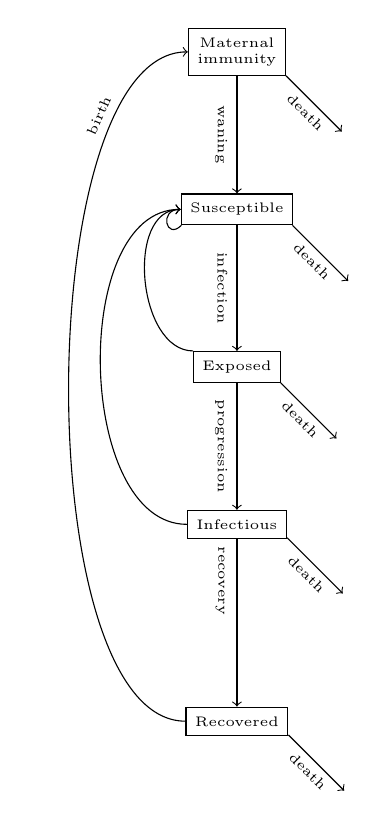
\begin{tikzpicture}[compartment/.style = {rectangle, draw}, font=\fontsize{5pt}{6}\selectfont]
  % Compartments.
  \node at (0, 11) [compartment, align=center, name=MaternalImmunity] {Maternal\\immunity};
  \node at (0, 9) [compartment, name=Susceptible] {Susceptible};
  \node at (0, 7) [compartment, name=Exposed] {Exposed};
  \node at (0, 5) [compartment, name=Infectious] {Infectious};
  \node at (0, 2.5) [compartment, name=Recovered] {Recovered};

  % Location for branch from Infectious to Chronic and Recovered.
  \coordinate (recovery) at (0, 3.75);

  % Infection-related processes.
  \draw [->] (MaternalImmunity)
             to node [rotate=-90, below] {waning}
             (Susceptible);
  \draw [->] (Susceptible)
             to node [rotate=-90, below] {infection}
             (Exposed);
  \draw [->] (Exposed)
             to node [rotate=-90, below] {progression}
             (Infectious);
  \draw [  ] (Infectious)
             to node [rotate=-90, below, yshift=-1pt] {recovery}
             (recovery);
  \draw [->] (recovery)
             to node [] {}
             (Recovered.90);

  % Births
  \draw [->] (Susceptible.196)
             to [out=225, in=180, looseness=3.5] node [] {}
             (Susceptible.180);
  \draw [->] (Exposed.160)
             to [out=180, in=180] node [] {}
             (Susceptible.180);
  \draw [->] (Infectious.180)
             to [out=180, in=180, looseness=0.9] node [sloped, above, pos=0.85] {}
             (Susceptible.180);
  \draw [->] (Recovered.180)
             to [out=180, in=180, looseness=0.6] node [sloped, above, pos=0.8] {birth}
             (MaternalImmunity.180);

  % Deaths
  \draw [->] (MaternalImmunity.334)
             to node [sloped, below, yshift=1pt] {death}
             +(315: 1);
  \draw [->] (Susceptible.344)
             to node [sloped, below, yshift=1pt] {death}
             +(315: 1);
  \draw [->] (Exposed.340)
             to node [sloped, below, yshift=1pt] {death}
             +(315: 1);
  \draw [->] (Infectious.345)
             to node [sloped, below, yshift=1pt] {death}
             +(315: 1);
  \draw [->] (Recovered.345)
             to node [sloped, below, yshift=1pt] {death}
             +(315: 1);
\end{tikzpicture}

%%% Local Variables:
%%% mode: latex
%%% TeX-master: "diagram_standalone"
%%% End:

  \caption{Model diagram.  Death from each state is not shown.}
  \label{fig:diagram}
\end{figure}


The simulations follow a Gillespie algorithm \citep{gillespie_1977}.
For each buffalo, a list of events and the times they occur is stored.
The next event over the whole population is found and the population
is updated.  The hazards for infection depend on the number of
infectious buffalo in the population and so the times to infection are
updated after each change in the population.  The hazards of the other
events are independent of the state of the population and so the times
to these events are not updated.  This process was repeated from $t =
0$ to $t = t_{\text{max}}$ or until there were $0$ infected (exposed,
infectious, and chronic) buffalo.

When sampling from simple distributions, standard algorithms were used
\citep{scipy}.  For complex distributions, the event times were
sampled using the inverse transform method \citep{rubinstein_1981}.

The variables $t$ and $a$ denote time and age, respectively, and are
both in units of years.

\section{Death}

We took the annual survival to be
\begin{equation}
  \Prob\{\text{Survival for $\unit[1]{yr}$}\}
  =
  \begin{cases}
    0.66 & \text{if $a < 1$},
    \\
    0.79 & \text{if $1 \leq a < 3$},
    \\
    0.88 & \text{if $3 \leq a < 12$},
    \\
    0.66 & \text{if $a \geq 12$}.
  \end{cases}
\end{equation}
Assuming that the mortality hazard is constant throughout a year gives
the hazard
\begin{equation}
  h_{\text{mortality}}(a)
  = - \log \Prob\{\text{Survival for $\unit[1]{yr}$}\},
\end{equation}
and the survival
\begin{equation}
  \begin{split}
    S_{\text{mortality}}(a)
    =
    \begin{cases}
      0.66^a
      & \text{if $a < 1$},
      \\
      0.66 \cdot 0.79^{a - 1}
      & \text{if $1 \leq a < 3$},
      \\
      0.66 \cdot 0.79^2 \cdot 0.88^{a - 3}
      & \text{if $3 \leq a < 12$},
      \\
      0.66 \cdot 0.79^2 \cdot 0.88^9 \cdot 0.66^{a - 12}
      & \text{if $a \geq 12$}.
    \end{cases}
  \end{split}
\end{equation}


\section{Birth}

We assumed that females reach reproductive maturity at age $4$ and
that the birth hazard varies at a periodic, triangular-shaped rate in
time:
\begin{equation}
  h_{\text{birth}}(t, a) =
  \begin{cases}
    0 & \text{if $a < 4$},
    \\
    \mu \alpha \max\big(1 - \beta (1 - |1 - 2 \{t - \tau\}|), 0\big)
    & \text{if $a \geq 4$},
  \end{cases}
\end{equation}
with
\begin{equation}
  \alpha =
  \begin{cases}
    1 + c_{\text{v}} \sqrt{3}
    & \text{if $c_{\text{v}} < \frac{1}{\sqrt{3}}$},
    \\
    \frac{3}{2} \left(1 + c_{\text{v}}^2\right)
    & \text{if $c_{\text{v}} \geq \frac{1}{\sqrt{3}}$},
  \end{cases}
\end{equation}
\begin{equation}
  \beta =
  \begin{cases}
    \frac{2 c_{\text{v}} \sqrt{3}}{1 + c_{\text{v}} \sqrt{3}}
    & \text{if $c_{\text{v}} < \frac{1}{\sqrt{3}}$},
    \\
    \frac{3}{4} \left(1 + c_{\text{v}}^2\right)
    & \text{if $c_{\text{v}} \geq \frac{1}{\sqrt{3}}$},
  \end{cases}
\end{equation}
and $\{x\}$ is the fractional part of $x$
(\autoref{fig:birth_hazard}).  The magnitude of the seasonal variation
is captured by the coefficient of variation $c_{\text{v}}$.  The time of year
of the peak birth hazard is $\tau$.  The annual mean $\mu$ was chosen
so that the population achieves the mean growth rate $r = 0$.  (See
\autoref{stable_age_structure}.)

\begin{figure}
  \centering
  \input{birth_hazard.pgf}
  \caption{Model birth hazards for ages 4 years and older.}
  \label{fig:birth_hazard}
\end{figure}

The cumulative hazard for $t$ years, given age $a_0$ at the current
time $t_0$ is
\begin{equation}
  H_{\text{birth}}(t, t_0, a_0) =
  \begin{cases}
    0 & \text{if $a_0 + t < 4$},
    \\
    \mu \left(H_0 + H_1  + H_2\right)
    & \text{if $a_0 + t \geq 4$ and $c_{\text{v}} < \frac{1}{\sqrt{3}}$},
    \\
    \mu \left(H_0 + H_3 + H_4\right)
    & \text{if $a_0 + t \geq 4$ and $c_{\text{v}} \geq \frac{1}{\sqrt{3}}$},
  \end{cases}
\end{equation}
with
\begin{equation}
  \begin{split}
    c &= t_0 + \max(4 - a_0, 0) - \tau,
    \\
    d &= t_0 + t - \tau,
    \\
    H_0 &= \lfloor d \rfloor - \lfloor c \rfloor - 1,
    \\
    H_1 &=
    \begin{cases}
      \frac{1}{2}
      + \alpha \left(\frac{1}{2} - \{c\}\right)
      \left[1 - \beta
        + \beta \left(\frac{1}{2} - \{c\}\right)\right]
      & \text{if $\{c\} < \frac{1}{2}$},
      \\
      \alpha \left(1 - \{c\}\right)
      \left[1 - \beta + \beta \left(1 - \{c\}\right)\right]
      & \text{if $\{c\} \geq \frac{1}{2}$},
    \end{cases}
    \\
    H_2 &=
    \begin{cases}
      \alpha \{d\}\left(1 - \beta \{d\}\right)
      & \text{if $\{d\} < \frac{1}{2}$},
      \\
      \frac{1}{2}
      + \alpha \left(\{d\} - \frac{1}{2}\right)
      \left[1 - \beta
        + \beta \left(\{d\} - \frac{1}{2}\right)\right]
      & \text{if $\{d\} \geq \frac{1}{2}$},
    \end{cases}
    \\
    H_3 &=
    \begin{cases}
      \frac{1}{2} + \alpha \beta \left(\frac{1}{2 \beta} - \{c\}\right)^2
      & \text{if $\{c\} < \frac{1}{2 \beta}$},
      \\
      \frac{1}{2}
      & \text{if $\frac{1}{2 \beta} \leq \{c\} < 1 - \frac{1}{2 \beta}$},
      \\
      \alpha \left(1 - \{c\}\right) \left[1 -
        \beta \left(1 - \{c\}\right)\right]
      & \text{if $\{c\} \geq 1 - \frac{1}{2 \beta}$},
    \end{cases}
    \\
    H_4 &=
    \begin{cases}
      \alpha \{d\} \left[1 - \beta \{d\}\right]
      & \text{if $\{d\} < \frac{1}{2 \beta}$},
      \\
      \frac{1}{2}
      & \text{if $\frac{1}{2 \beta} \leq \{d\} <
        1 - \frac{1}{2 \beta}$},
      \\
      \frac{1}{2}
      + \alpha \beta
      \left[\{d\} - \left(1 - \frac{1}{2 \beta}\right)\right]^2
      & \text{if $\{d\} \geq 1 - \frac{1}{2 \beta}$},
    \end{cases}
  \end{split}
\end{equation}
and $\lfloor x \rfloor$ is the floor function,
i.e.~$\lfloor x \rfloor = x - \{x\}$.
The survival function for $t$ years, given age
$a_0$ at the current time $t_0$ is then
\begin{equation}
  S_{\text{birth}}(t, t_0, a_0) = \exp\left(- H_{\text{birth}}(t, t_0, a_0)\right).
\end{equation}
The probability density function for births time $t$ later, given age
$a_0$ at $t_0$, is
\begin{align}
  f_{\text{birth}}(t, t_0, a_0) =
  h_{\text{birth}}(t_0 + t, a_0 + t)
  S_{\text{birth}}(t, t_0, a_0).
\end{align}

% Multiplying the probability density by $N(t_0, a_0)$, the density of
% females aged $a_0$ at $t_0$, and integrating over $a_0$ gives the
% expected number of births time $t$ later:
% \begin{equation}
%   b(t, t_0) = \int_0^{\infty} f_{\text{birth}}(t, t_0, a_0) N(t_0, a_0) \md a_0.
% \end{equation}
% Binning by month gives the expected number of births in month $m$:
% \begin{align}
%   g(m, t_0) &=
%   \int_0^1 b\left(\frac{m + \mu}{12}, t_0\right) \md \mu
%   & & \text{for $m \in \{0, 1, 2, \ldots\}$}.
% \end{align}

On birth, the newborn is female with probability
$p_{\text{female birth}} = 0.5$ or otherwise male.


\section{Waning}

The duration of maternal immunity was taken to be a standard gamma
random variable with shape $k_{\text{maternal immunity}}$
and mean $\mu_{\text{maternal immunity}}$.


\section{Infection}

The infection hazard was taken to be
\begin{equation}
  h_{\text{infection}}(t) = \beta_{\text{acute}} I(t) +
  \beta_{\text{chronic}} C(t),
\end{equation}
where $I(t)$ and $C(t)$ are the total number of infectious and
chronic-carrier buffalo in the herd at time $t$.  Over periods where
$I(t)$ and $C(t)$ are constant, the hazard is constant, which gives an
exponential random variable.


\section{Progression}

The duration of the latent period was taken to be a standard gamma
random variable with shape $k_{\text{progression}}$
and mean $\mu_{\text{progression}}$.


\section{Recovery}

The duration of infection was taken to be a standard gamma random
variable with shape $k_{\text{recovery}}$ and mean
$\mu_{\text{recovery}}$.

On recovery, buffalo become chronic carriers with probability
$p_{\text{chronic}}$ or otherwise is recovered, i.e.~fully cleared
of pathogen.


\section{Chronic recovery}

The duration of the chronic-carrier state was taken to be an
exponential random variable with mean
$\mu_{\text{chronic recovery}}$.


\section{Initial conditions}

A sample of size $N$ from the stable age structure was used to
initialize the population.  (See \autoref{stable_age_structure}.)  The
sex of each buffalo was randomly selected with probability
$p_{\text{female birth}}$ of being female.
% The simulations were started at $t = 0$ with $2$ initial infections
% in randomly chosen members of the population.


\begin{figure}
  \centering
  \input{distributions.pgf}
  \caption{Hazards and survivals for the model events.
    \textbf{Add stable age distribution?}}
  \label{fig:distributions}
\end{figure}


\section{Stable age structure}
\label{stable_age_structure}

The mean rate of female births $B(t)$ follows the Lotka equation
\begin{equation}
  \label{lotka}
  \begin{split}
    B(t) =&
    p_{\text{female birth}} \bigg[
      \int_0^t B(t - a)
      S_{\text{mortality}}(a)
      h_{\text{birth}}(t, a) \md a
    \\
    & \quad\quad\quad\quad\quad {} +
      \int_0^{\infty} n_0(a)
      \frac{S_{\text{mortality}}(a + t)}{S_{\text{mortality}}(a)}
      h_{\text{birth}}(t, a + t) \md a
    \bigg],
  \end{split}
\end{equation}
where $n_0(a)$ is the density of age $a$ females at time $t = 0$
\citetext{\citealp[Chapter VI, Section 29 on
  pp.~159--161]{harris_1963};
  \citealp[Chapter 20 on pp.~353--364]{kot_01}}.
% For large $t$, the contribution of the initial cohort---the second
% integral in \eqref{lotka}---becomes negligible, so
% \begin{equation}
%   B(t) =
%   p_{\text{female birth}} \int_0^t B(t - a)
%   \hat{h}_{\text{birth}}(t, a) \md a
% \end{equation}
% for large $t$,
% where
% \begin{equation}
%   \hat{h}_{\text{birth}}(t, a) =
%   S_{\text{mortality}}(a)
%   h_{\text{birth}}(t, a).
% \end{equation}
% Alternately,
% \begin{equation}
%   B(t)
%   =
%   p_{\text{female birth}} \int_0^{t}
%   B(u)
%   \hat{h}_{\text{birth}}(t, t - u)
%   \md u.
% \end{equation}
Given $B(t)$, the mean density of females of age $a$ is
\begin{equation}
  n(t, a) =
  \begin{cases}
    B(t - a) S_{\text{mortality}}(a)
    & \text{if $a < t$},
    \\
    n_0(a - t)
    \frac{S_{\text{mortality}}(a)}{S_{\text{mortality}}(a - t)}
    & \text{if $a > t$}.
  \end{cases}
\end{equation}
The mean density of females of age $a$ satisifies the McKendrick--von
Foerster equation
\begin{equation}
  \begin{split}
    \frac{\partial n}{\partial t} + \frac{\partial n}{\partial a}
    &= - h_{\text{death}}(a) n(t, a),
    \\
    n(t, 0) &=
    p_{\text{female birth}}
    \int_0^{+\infty} n(t, a) h_{\text{birth}}(t, a) \md a,
    \\
    n(0, a) &= n_0(a).
  \end{split}
\end{equation}

\comment{Crank--Nicolson on characteristics, after \citep{milner_1992}.}

Discretizing in $a$ by setting
\begin{equation}
  \vec{a}
  = \left[0, \Delta a, 2 \Delta a, \cdots, a_{\text{max}} \right]^{\mT}
\end{equation}
and
\begin{equation}
  \vec{n}(t) \approx n(t, \vec{a})
\end{equation}
gives
\begin{equation}
  \label{ODE}
  \frac{\md \vec{n}}{\md t}
  = \big(\mat{B}(t) + \mat{T}\big) \vec{n}(t),
\end{equation}
with
\begin{equation}
  \begin{split}
    \mat{B}(t)
    &= p_{\text{female birth}}
    \begin{bmatrix}
      \cdots & h_{\text{birth}}(t, \vec{a}) & \dots
      \\
      \cdots & 0 & \cdots
      \\
      \cdots & 0 & \cdots
      \\
      & \vdots &
      \\
      \cdots & 0 & \cdots
    \end{bmatrix},
    \\
    \mat{T}
    &= \mat{M} + \mat{A},
    \\
    \mat{M}
    &= \operatorname{diag}\left(- h_{\text{mortality}}(\vec{a})\right),
    \\
    \mat{A}
    &= \frac{1}{\Delta a}
    \begin{bmatrix}
      -1 & 0 & 0 & 0 & \cdots & 0 & 0
      \\
      1 & -1 & 0 & 0 & \cdots & 0 & 0
      \\
      0 & 1 & -1 & 0 & \cdots & 0 & 0
      \\
      \vdots & \ddots & \ddots & \ddots & \ddots &  & \vdots
      \\
      \vdots &  & \ddots & \ddots & \ddots & \ddots & \vdots
      \\
      0  & \cdots & \cdots & 0 & 1 & - 1 & 0
      \\
      0  & \cdots & \cdots & \cdots & 0 & 1 & 0
    \end{bmatrix}.
  \end{split}
\end{equation}

The monodromy matrix $\mat{\Phi}(T)$ of the ODE approximation
\eqref{ODE} satisfies
\begin{equation}
  \begin{split}
    \frac{\md \mat{\Phi}}{\md t}
    &= \big(\mat{B}(t) + \mat{T}\big) \mat{\Phi}(t),
    \\
    \mat{\Phi}(0) &= \mat{I},
  \end{split}
\end{equation}
where $\mat{I}$ is the identity matrix and the period $T = \unit[1]{y}$
is the period of $\mat{B}(t)$ \citep{parker_1992}.
The monodromy matrix projects the population forward at integer
multiples of the period:
\begin{align}
  \vec{n}(k T) &= \big[\mat{\Phi}(T)\big]^k \vec{n}(0),
  & \text{for $k = 0, 1, 2, \ldots$}.
\end{align}
The dominant eigenvalue $\rho_0$ of $\mat{\Phi}(T)$, i.e.~the
eigenvalue with largest magnitude, gives the population growth rate
\begin{equation}
  r = \frac{1}{T} \log \rho_0,
\end{equation}
and the corresponding right eigenvector is the stable age structure.

We numerically computed the population growth rate and stable age
structure by using age steps $\Delta a = 0.01$,
maximum age $a_{\text{max}} = 25$
(probability of survival $S_{\text{mortality}}(25) \approx 0.0006$),
finding the monodromy matrix by numerically solving \eqref{ODE}, and
then finding its dominant eigenvalue and corresponding eigenvector.
We then used a root-finding algorithm to find the value of the mean
birth hazard $\mu \approx 0.9915$ that gave growth rate $r = 0$.
Halving the age step to $\Delta a = 0.005$
gave a relative error for $\mu$ of $8 \times 10^{-4}$
and doubling the maximum age to $a_{\text{max}} = 50$
gave a relative error of $5 \times 10^{-9}$.
These computations were done in Python 3.6.5 \citep{python} using the
NumPy \citep{numpy} and SciPy \citep{scipy} libraries.


\bibliography{journal_abbreviations,math_epi}
\bibliographystyle{jpmbib}


\end{document}
